\subsection{Chapter 6 - Applying Newton's Laws}

\subsubsection{Overview}\label{chap:ApplyingNewtonsLaws}

In this chapter, we take a closer look at how to use Newton's Laws to build models to describe motion. Whereas the previous chapter was focused on identifying the forces that are acting on an object, this chapter focuses on using those forces to describe the motion of the object.

Newton's Laws are meant to describe ``point particles'', that is, objects that can be thought of as a point and thus have no orientation. A block sliding down a hill, a person on a merry-go-round, a bird flying through the air can all be modelled as point particles, as long as we do not need to model their orientation. In all of these cases, we can model the forces on the object using a free-body diagram as the location of where the forces are applied on the object do not matter. In later chapters, we will introduce the tools required to apply Newton's Second Law to objects that can rotate, where we will see that the location of where a force is exerted matters.

\begin{framed}
\textbf{Learning Objectives}\\
\begin{itemize}
\item Understand when an object's motion can be modelled as one dimensional (linear).
\item Be able to develop models for objects undergoing linear motion.
\item Be able to develop models for objects undergoing circular motion.
\item Be able to develop models for objects undergoing arbitrary three dimensional motion.
\item Understand the forces involved in circular motion, and understand that ``centripetal'' and ``centrifugal'' forces are not really forces.
\end{itemize}
\end{framed}

\begin{framed}
\textbf{Think About It}\\
If a person swings on a swing where the ropes are damaged, where are the ropes most likely to break?

\begin{enumerate}
\item at the bottom of the trajectory, when the speed is the greatest.
\item at the top of the trajectory, when the speed is zero.
\item at the point in the trajectory where the speed is one half of its maximal value.
\end{enumerate}

\begin{framed}
\textbf{Answer}\\
\begin{enumerate}
\item
\end{enumerate}
\end{framed}
\end{framed}

\subsubsection{Statics}

When using Newton's Laws to model an object, one can identify two broad categories of situations: static and dynamic. In static situations, the acceleration of the object is zero. By Newton's Second Law, this means that the vector sum of the forces (and torques, as we will see in a later chapter) exerted on an object must be zero. In dynamic situations, the acceleration of the object is non-zero.

For static problems, since the acceleration vector is zero, we can choose a coordinate system in a way that results in as many forces as possible being aligned with the axes (so that we minimize the number of forces that we need to break up into components).

\begin{framed}
\textbf{Example 6.1}\\
You push horizontally with a force $\vec F$ on a box of mass $m$ that is resting against a vertical wall, as shown in Figure~\ref{fig:applyingnewtonslaws:blockwall}. The coefficient of static friction between the wall and the box is $\mu_s$. What is the minimum magnitude of the force that you must exert for the box to remain stationary?

\begin{figure}[!htbp]
\centering
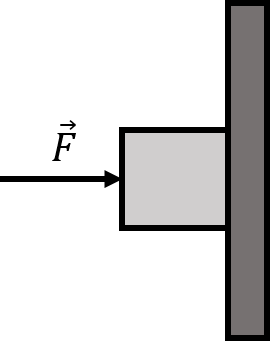
\includegraphics[width=0.2\linewidth]{files/blockwall-4c9d39aeb582ba18ba06ff1f9b6bb5dc.png}
\caption[]{A horizontal force exerted on box that is resting against a wall.}
\label{fig:applyingnewtonslaws:blockwall}
\end{figure}

\begin{framed}
\textbf{Solution}\\
Since the acceleration of the box is zero, the vector sum of the forces exerted on the box is zero. We start by identifying the forces exerted on the box; these are:

\begin{enumerate}
\item $\vec F$, the horizontal force that you exert on the box.
\item $\vec F_g$, the weight of the box, with magnitude $mg$.
\item $\vec N$, a normal force exerted by the wall on the box. The force is in the horizontal direction, in the opposite direction to $\vec F$.
\item $\vec f_s$, a vertical force of static friction between the wall and the box. The force points upwards as the ``impeding motion'' of the block is downwards. The force will have at most a magnitude of $f_s\leq\mu_s N$, since the force of static friction depends on the other forces exerted on the object.
\end{enumerate}

The forces are shown in the free-body diagram in Figure~\ref{fig:applyingnewtonslaws:blockwall_fbd}, along with our choice of coordinate system which was chosen so that all forces are either in the $x$ or $y$ direction.

\begin{figure}[!htbp]
\centering
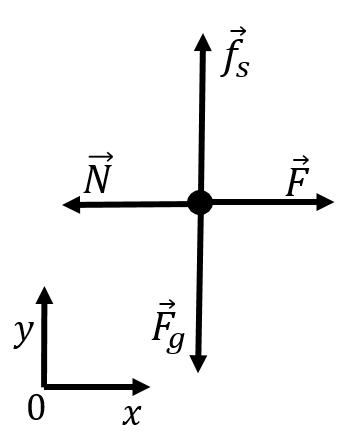
\includegraphics[width=0.25\linewidth]{files/blockwall_fbd-d828b9d9bae419f4ebd6743c00c86c4f.png}
\caption[]{Free-body diagram of the forces exerted on the box.}
\label{fig:applyingnewtonslaws:blockwall_fbd}
\end{figure}

The $x$ component of Newton's Second Law is:
\begin{equation}
\sum F_x = F - N &=0\\
\therefore N = F
\end{equation}
which tells us that the normal force exerted by the wall has the same magnitude as the applied force, $\vec F$. The $y$ component of Newton's Second Law is:
\begin{equation}
\sum F_y = f_s - F_g &=0\\
\therefore f_s -mg &=0\\
\therefore f_s = mg\\
\end{equation}
which tells us that the force of friction must have the same magnitude as the weight. This makes sense, since they are the only forces with components in the $y$ direction, and thus, they must cancel each other out.

The force of friction will be less than or equal to $\mu_sN$, and thus less than or equal to $\mu_s F$, since $\vec F$ and $\vec N$ have the same magnitude (from the $x$ component of Newton's Second Law). Furthermore, since $f_s=mg$, we can write:
\begin{equation}
f_s &\leq \mu_s F\\
\therefore mg &\leq \mu_s F\\
\therefore \frac{mg}{\mu_s} &\leq F
\end{equation}
which gives us the condition that $F\geq mg/\mu_s$, and thus the minimum magnitude of $F$ in order to keep the box from sliding down.

Although we used the lesser than or equal to sign in the above equations, we could have used an equal sign if we were confident that the force of friction has its maximal magnitude, $f_s=\mu_sN$. The maximal magnitude of the force of friction is proportional to the force that we exert (since $N=F$); if we want to exert the least amount of force $F$, then we need the force of friction to be equal to its maximal magnitude which needs to be equal to the weight of the box.

\textbf{Discussion:} This model for the minimal required force makes sense because:

\begin{itemize}
\item The dimension of $mg/\mu_s$ is force.
\item If the mass of the box is increased, then one needs to push harder against the box to keep it up.
\item If the coefficient of static friction, $\mu_s$, is increased, one does not need to push as hard.
\end{itemize}
\end{framed}
\end{framed}

\subsubsection{Linear motion}

We can describe the motion of an object whose \textit{velocity vector does not continuously change direction} as ``linear'' motion. For example, an object that moves along a straight line in a particular direction, then abruptly changes direction and continues to move in a straight line can be modelled as undergoing linear motion over two different segments (which we would model individually). An object moving around a circle, with its velocity vector continuously changing direction, would not be considered to be undergoing linear motion. For example, paths of objects undergoing linear and non-linear motion are illustrated in Figure~\ref{fig:applyingnewtonslaws:linearmotion}.

\begin{figure}[!htbp]
\centering
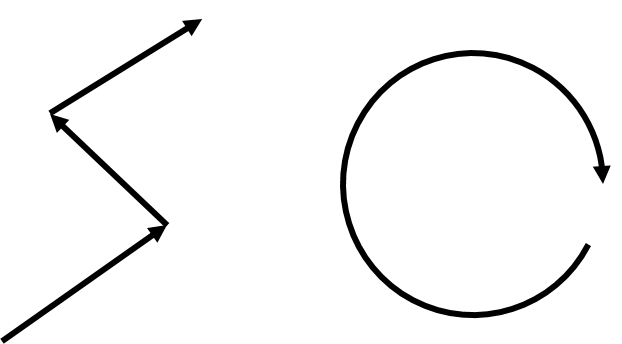
\includegraphics[width=0.3\linewidth]{files/linearmotion-3c36fb7975de9f562924e0686e09b329.png}
\caption[]{(Left:) Displacement vectors for an object undergoing three segments that can each be modelled as linear motion. (Right:) Path of an object whose velocity vector changes continuously and cannot be considered as linear motion.}
\label{fig:applyingnewtonslaws:linearmotion}
\end{figure}

When an object undergoes linear motion, we always model the motion of the object over straight segments separately. Over one such segment, the acceleration vector will be co-linear with the displacement vector of the object (parallel or anti-parallel - note that the acceleration can change direction as it would from a spring force, but will always be co-linear with the displacement).

\begin{framed}
\textbf{Example 6.2}\\
A block of mass $m$ is placed at rest on an incline that makes an angle $\theta$ with respect to the horizontal, as shown in Figure~\ref{fig:applyingnewtonslaws:blockI}. The block is nudged slightly so that the force of static friction is overcome and the block starts to accelerate down the incline. At the bottom of the incline, the block slides on a horizontal surface.

The coefficient of kinetic friction between the block and the incline is $\mu_{k1}$, and the coefficient of kinetic friction between the block and horizontal surface is $\mu_{k2}$. If one assumes that the block started at rest a distance $L$ from the bottom of the incline, how far along the horizontal surface will the block slide before stopping?

\begin{figure}[!htbp]
\centering
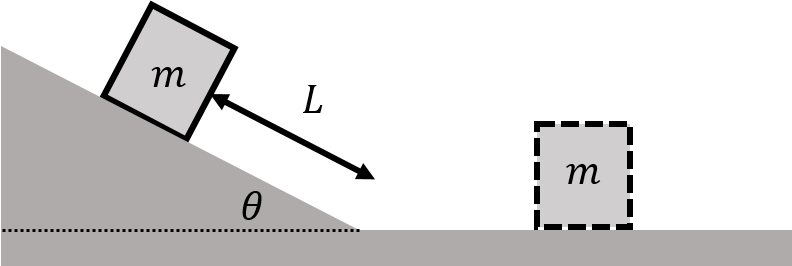
\includegraphics[width=0.5\linewidth]{files/blockI-196266707a8dcc96b8022966b7a2e44b.png}
\caption[]{A block slides down an incline before sliding on a flat surface and stopping.}
\label{fig:applyingnewtonslaws:blockI}
\end{figure}

\begin{framed}
\textbf{Solution}\\
We can identify that this is linear motion that we can break up into two segments: (1) the motion down the incline, and (2), the motion along the horizontal surface. We will thus identify the forces, draw the free-body diagram for the block, and use Newton's Second Law twice, once for each segment.

It is often useful to describe the motion in words to help us identify the steps required in building a model for the block. In this case we could say that:

\begin{enumerate}
\item The block slides down the incline and accelerates in the direction of motion. By identifying the forces and applying Newton's Second Law, we can determine its acceleration which will be parallel to the incline.
\item The block will reach a certain speed at the bottom of the incline, which we can determine from kinematics by knowing that the block travelled a distance $L$, with a known acceleration and that it started at rest.
\item The block will decelerate along the horizontal surface. Again, by identifying the forces and using Newton's Second Law, we will be able to determine the acceleration of the block.
\item The block will stop after having travelled an unknown distance, which we can find by using kinematics and knowing the acceleration of the block as well as its initial velocity at the bottom of the incline.
\end{enumerate}

Our first step is thus to identify the forces on the block while it is on the incline. These are:

\begin{enumerate}
\item $\vec F_{g}$, its weight.
\item $\vec N_1$, a normal force exerted by the incline.
\item $\vec f_{k1}$, a force of kinetic friction exerted by the incline. The force is opposite of the direction of motion, and has a magnitude given by $f_{k1}=\mu_{k1}N_1$.
\end{enumerate}

These are shown on the free-body diagram in Figure~\ref{fig:applyingnewtonslaws:blockI_fbd1}. As usual, we drew the acceleration, $\vec a_1$, on the free-body diagram, and chose the direction of the $x$ axis to be parallel to the acceleration.

\begin{figure}[!htbp]
\centering
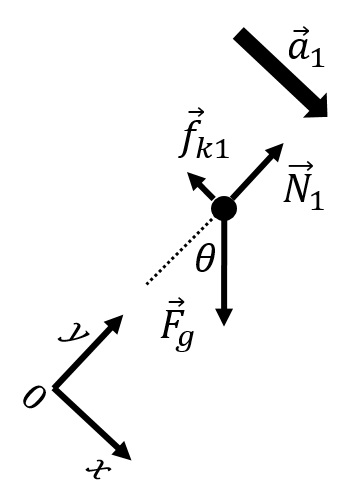
\includegraphics[width=0.25\linewidth]{files/blockI_fbd1-ef908fa1c7223f0c653ddd2f630b7890.png}
\caption[]{Free-body diagram for the block when it is on the incline.}
\label{fig:applyingnewtonslaws:blockI_fbd1}
\end{figure}

Writing out the $x$ component of Newton's Second Law, and using the fact that the acceleration is in the $x$ direction ($\vec a=a_1\hat x$):
\begin{equation}
\sum F_x = F_g\sin\theta - f_{k1} &= ma_1\\
\therefore mg\sin\theta - \mu_{k1} N_1 &= ma_1
\end{equation}
where we expressed the magnitude of the kinetic force of friction in terms of the normal force exerted by the plane, and the weight in terms of the mass and gravitational field, $g$. The $y$ component of Newton's Second Law can be written:
\begin{equation}
\sum F_y = N_1-F_g\cos\theta &= 0\\
\therefore N_1 = mg\cos\theta
\end{equation}
which we used to express the normal force in terms of the weight. We can use this expression for the normal force by substituting it into the equation we obtained from the $x$ component to find the acceleration along the incline:
\begin{equation}
mg\sin\theta - \mu_{k1} N_1 &= ma_1\\
mg\sin\theta - \mu_{k1} mg\cos\theta&= ma_1\\
\therefore a_1 &= g(\sin\theta-\mu_{k1}\cos\theta)
\end{equation}
Now that we know the acceleration down the incline, we can easily find the velocity at the bottom of the incline using kinematics. We choose the origin of the $x$ axis to be zero where the block started ($x_0=0$), so that the block is at position $x=L$ at the bottom of the incline. Using kinematics, we can find the speed, $v$, given that the initial speed, $v_0=0$:
\begin{equation}
v^2-v_0^2&=2a_1(x-x_0)\\
v^2&=2a_1L\\
\therefore v &= \sqrt{2a_1L}\\
&=\sqrt{2Lg(\sin\theta-\mu_{k1}\cos\theta)}
\end{equation}
We can now proceed to build a model for the second segment. We first identify the forces on the block when it is on the horizontal surface; these are:

\begin{enumerate}
\item $\vec F_{g1}$, its weight.
\item $\vec N_2$, a normal force exerted by the horizontal surface. This is in general different than the normal force exerted when the block was on the inclined plane.
\item $\vec f_{k2}$, a force of kinetic friction exerted by the horizontal surface. The force is opposite of the direction of motion, and has a magnitude given by $f_{k2}=\mu_{k2}N_2$.
\end{enumerate}

The forces are illustrated by the free-body diagram in Figure~\ref{fig:applyingnewtonslaws:blockI_fbd2}, where we showed the acceleration vector, $\vec a_2$, which we determined to be to the left since the block is decelerating. We also chose an $xy$ coordinate system such that the $x$ axis is anti-parallel to the acceleration, so that the motion is in the positive $x$ direction (and the acceleration in the negative $x$ direction).

\begin{figure}[!htbp]
\centering
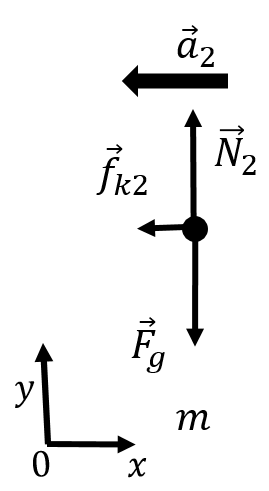
\includegraphics[width=0.2\linewidth]{files/blockI_fbd2-4e6e287ceddbf63637b8634847bdfa7f.png}
\caption[]{Free-body diagram for the block when it is sliding along the horizontal surface. We (arbitrarily) chose the positive $x$ direction to be in the direction of motion and anti-parallel to the acceleration. We could easily have chosen the opposite direction.}
\label{fig:applyingnewtonslaws:blockI_fbd2}
\end{figure}

Writing out the $x$ component of Newton's Second Law:
\begin{equation}
\sum F_x = -f_{k2} &= -ma_2\\
\therefore \mu_{k2}N_2 &= ma_2
\end{equation}
where we expressed the force of kinetic friction using the normal force. We  have to be careful here with the sign of the acceleration; the equation that we wrote implies that $a_2$ is a positive number, since $\mu_{k2}$ is positive and $N_2$ is also positive (it is the magnitude of the normal force). $a_2$ is the magnitude of the acceleration, and we included the fact that the acceleration points in the negative $x$ direction when we put a negative sign in the first line. The $x$ component of the acceleration is $-a_2$, and the vector is given by $\vec a_2= -a_2\hat x$.

The $y$ component of Newton's Second Law will allow us to find the normal force:
\begin{equation}
\sum F_y = N_2 -F_g &=0\\
\therefore N_2 = mg
\end{equation}
which we can substitute back into the $x$ equation to find the magnitude of the acceleration along the horizontal surface:
\begin{equation}
ma_2 &=\mu_{k2}N_2 \\
\therefore a_2&=\mu_{k2}g
\end{equation}
Now that we have found the acceleration along the horizontal surface, we can use kinematics to find the distance that the block travelled before stopping. We choose the origin of the $x$ axis to be the bottom of the incline ($x_0=0$), the acceleration is negative $a_x = -a_2 = -mu_{k2}g$, the final speed is zero, $v=0$, and the initial speed, $v_0$ is given by our model for the first segment. Using one of the kinematic equations:
\begin{equation}
v^2-v_0^2&=2(-a_2)(x-x_0)\\
v_0^2&=2a_2x\\
\therefore x &=\frac{1}{2a_2}v_0^2\\
&=\frac{1}{2\mu_{k2}g}2Lg(\sin\theta-\mu_{k1}\cos\theta)\\
\therefore x&=\frac{(\sin\theta-\mu_{k1}\cos\theta)}{\mu_{k2}}L
\end{equation}
\textbf{Discussion:} The model for the distance $x$ that it takes the block to stop makes sense because:

\begin{itemize}
\item All of the terms in the fraction are dimensionless, so the value of $x$ will have the same dimension as $L$.
\item If we make $L$ bigger, then $x$ will be bigger (if we release the block from higher up on the incline, it will have more time to accelerate and will slide further before stopping).
\item If we make $\mu_{k1}$ bigger, then $x$ will be smaller: if we increase friction on the incline, the block will have a smaller acceleration and smaller speed at the bottom.
\item If we increase the friction with the horizontal plane (increase $\mu_{k2}$), then $x$ will be reduced (it won't slide as far if there is more friction on the horizontal plane).
\item If we increase $\theta$, the numerator will be larger, so $x$ will increase (the block will accelerate more down a steeper incline and end up further).
\end{itemize}
\end{framed}
\end{framed}

\begin{framed}
\textbf{Checkpoint}\\
A present is placed at rest on a plane that is inclined, at a distance $L$ from the bottom of the incline, much like the box in Example~6.2 above. At the bottom of the incline, the box is determined to have a speed $v$. If the box is instead released from a distance of $4L$ from the bottom of the incline, what will its speed at the bottom of the incline be?

\begin{enumerate}
\item $v$
\item $2v$
\item $4v$
\item it depends on the coefficient of friction between the present and the plane.
\end{enumerate}

\begin{framed}
\textbf{Answer}\\
\begin{enumerate}[resume]
\item
\end{enumerate}
\end{framed}
\end{framed}

\paragraph{Modelling situations where forces change magnitude}\label{sec:applyingnewtonslaws:modellingwhereforcechanges}

So far, the models that we have considered involved forces that remained constant in magnitude. In many cases, the forces exerted on an object can change magnitude and direction. For example, the force exerted by a spring changes as the spring changes length or the force of drag changes as the object changes speed. In these case, even if the object undergoes linear motion, we need to break up the motion into many small segments over which we can assume that the forces are constant. If the forces change continuously, we will need to break up the motion into an infinite number of segments and use calculus.

Consider the block of mass $m$ that is shown in Figure~\ref{fig:applyingnewtonslaws:blockvaryingforce}, which is sliding along a frictionless horizontal surface and has a  horizontal force $\vec F(x)$ exerted on it. The force has a different magnitude in the three segments of length $\Delta x$ that are shown. If the block starts at position $x=x_0$ axis with speed $v_0$, we can find, for example, its speed at position $x_3=3\Delta x$, after the block travelled through the three segments.

\begin{figure}[!htbp]
\centering
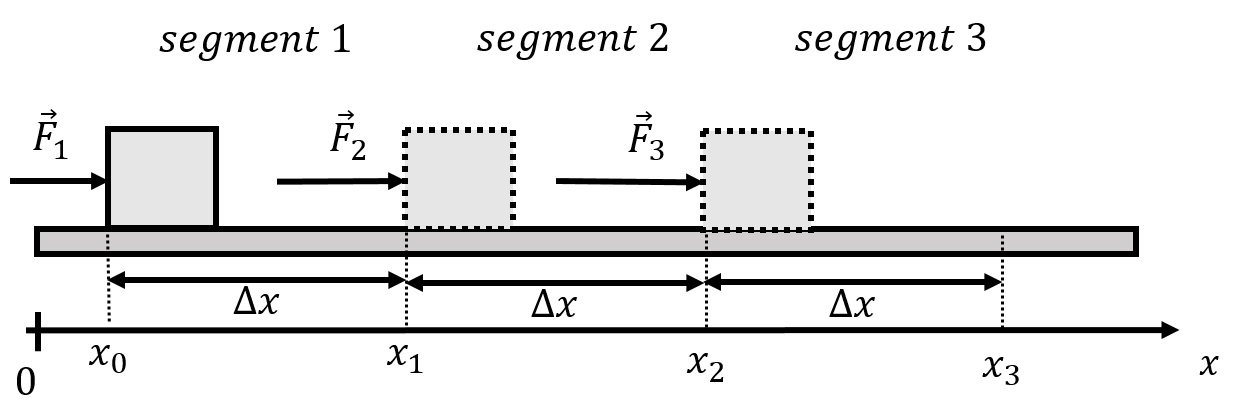
\includegraphics[width=0.7\linewidth]{files/blockvaryingforce-fcc0ef639c44cd3ed5e47cd858ad5a33.png}
\caption[]{A block being pushed along a frictionless horizontal surface with a force that changes.}
\label{fig:applyingnewtonslaws:blockvaryingforce}
\end{figure}

The horizontal force, $\vec F$, exerted on the block can be written as:
\begin{equation}
  \vec F (x)=
  \begin{cases}
    F_1\hat x & x<\Delta x \quad \text{(segment 1)}\\
    F_2\hat x & \Delta x \leq x< 2\Delta x \quad \text{(segment 2)}\\
    F_3\hat x & 2\Delta x \leq x\quad \text{(segment 3)}
  \end{cases}
\end{equation}
as it depends on the location of the block. To find the speed of the block at the end of the third segment, we can model each segment separately. The forces exerted on the block are the same in each segment:

\begin{enumerate}
\item $\vec F_g$, its weight, with magnitude $mg$.
\item $\vec N$, a normal force exerted by the ground.
\item $\vec F(x)$, an applied force that changes magnitude with position and is different in the three different segments.
\end{enumerate}

The forces are illustrated in the free-body diagram show in Figure~\ref{fig:applyingnewtonslaws:blockvaryingforce_fbd}.

\begin{figure}[!htbp]
\centering
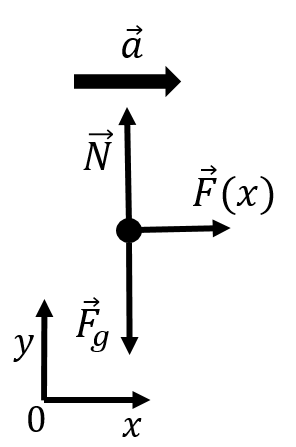
\includegraphics[width=0.2\linewidth]{files/blockvaryingforce_fb-f8568f60b83e0828429fe2eaf2c81104.png}
\caption[]{Free-body diagram for the block shown in Figure~\ref{fig:applyingnewtonslaws:blockvaryingforce}.}
\label{fig:applyingnewtonslaws:blockvaryingforce_fbd}
\end{figure}

Newton's Second Law can be used to determine the acceleration of the block for each of the three segments, since the forces are constant within one segment. For all three segments, the $y$ component of Newton's Second Law just tells us that the normal force exerted by the ground is equal in magnitude to the weight of the block. The $x$ component of Newton's Second Law gives the acceleration:
\begin{equation}
\sum F_x = F_i = ma_i
\end{equation}
where we have used the index $i$ to indicate which segment the block is in ($i$ can be 1, 2 or 3). The acceleration of the block in segment $i$ is given by:
\begin{equation}
a_i = \frac{F_i}{m}
\end{equation}
If the speed of the block is $v_0$ at the beginning of segment 1 ($x=x_0$), we can find its speed at the end of segment 1 ($x=x_1$), $v_1$, using kinematics and the fact that the acceleration in segment 1 is $a_1$:
\begin{equation}
v_1^2-v_0^2 &= 2a_1(x_1 - x_0)\\
v_1^2 &=v_0^2+ 2a_1\Delta x\\
\therefore v_1^2 &=v_0^2+2\frac{F_1}{m}\Delta x
\end{equation}
We can now easily find the speed at the end of segment 2 ($x=x_2$), $v_2$, since we know the speed at the beginning of segment 2 ($x_1$,$v_1$) and the acceleration $a_2$:
\begin{equation}
v_2^2 -v_1^2 &= 2a_2(x_2 - x_1)\\
\therefore v_2^2 &= v_1^2 + 2a_2\Delta x\\
&=v_0^2+ 2\frac{F_1}{m}\Delta x + 2\frac{F_2}{m}\Delta x
\end{equation}
It is easy to show that the speed at the end of the third segment is:
\begin{equation}
v_3^2 = v_0^2+ 2\frac{F_1}{m}\Delta x + 2\frac{F_2}{m}\Delta x +2\frac{F_3}{m}\Delta x
\end{equation}
If there were $N$ segments, with the force being different in each segment, we could use the summation notation to write:
\begin{equation}
v_N^2 &= v_0^2 + 2\sum_{i=1}^{i=N} \frac{F_i}{m}\Delta x
\end{equation}
Finally, if the magnitude of the force varied continuously as a function of $x$, $\vec F(x)$, we would model this by taking segments whose length, $\Delta x$, tends to zero (and we would need an infinite number of such segments). For example, if we wanted to know the speed of the object at position $x=X$ along the $x$ axis, with a force that was given by $\vec F(x)=F(x)\hat x$, if the object started at position $x_0$ with speed $v_0$, we would take the following limit:
\begin{equation}
v^2 = v_0^2 + \lim_{\Delta x \to 0} 2\sum_{i=1}^{i=N} \frac{F(x)}{m}\Delta x
\end{equation}
where $\Delta x = \frac{X}{N}$ so that as $\Delta x\to 0$, $N\to\infty$. Of course, integrals are the exact tool that allow us to evaluate the sum in this limit:
\begin{equation}
\lim_{\Delta x \to 0} 2\sum_{i=1}^{i=N} \frac{F_i}{m}\Delta x =2 \int_{x_0}^{X}\frac{F(x)}{m}dx
\end{equation}
and the speed at position $x=X$ is given by:
\begin{equation}
v^2 = v_0^2 + 2 \int_{x_0}^{X}\frac{F(x)}{m}dx
\end{equation}
Naturally, we can find the above result starting directly from calculus. If the component of the (net) force in the $x$ direction is given by $F(x)$, then the  acceleration is given by $a(x) = \frac{F(x)}{m}$. The velocity is related to the acceleration:
\begin{equation}
a(x) &= \frac{dv}{dt}\\
\therefore dv &= a(x)dt\\
\end{equation}
We cannot simply integrate the last equation to find that $v=\int a(x)dt$ because the acceleration is given as a function of position, $a(x)$, and not a function of time, $t$. Thus, we cannot simply take the integral over $t$ and must instead ``change variables'' to take the integral over $x$. $x$ and $t$ are related through velocity:
\begin{equation}
v &= \frac{dx}{dt}\\
\therefore dt &= \frac{1}{v}dx
\end{equation}
We can thus write:
\begin{equation}
dv &= a(x)dt = a(x)\frac{1}{v}dx \\
\end{equation}
The equation above is called a ``separable differential equation'', which can also be written:
\begin{equation}
\frac{dv}{dx}=\frac{1}{v}a(x)
\end{equation}
This is called a differential equation because it relates the derivative of a function (the derivative of $v$ with respect to $x$, on the left) to the function itself ($v$ appears on the right as well). The differential equation is ``separable'', because we can separate out all of the quantities that depend on $v$ and on $x$ on different sides of the equation:
\begin{equation}
vdv = a(x)dx
\end{equation}
This last equation says that $vdv$ is equal to $a(x)dx$. Remember that $dx$ is the length of a very small segment in $x$, and that $dv$ is the change in velocity over that very small segment. Since the terms on the left and right are equal, if we sum (integrate) the quantity $vdv$ over many segments, that sum must be equal to the sum (integral) of the quantity $a(x)dx$ over the same segments. Let us choose those segment such that for the beginning of the first interval the position and speed are $x_0$ and $v_0$, respectively, and the position and speed at the end of the last segment are $X$ and $V$, respectively. We then must have that:
\begin{equation}
\int_{v_0}^{V}vdv&=\int_{x_0}^{X}a(x)dx\\
 \frac{1}{2}V^2 - \frac{1}{2}v_0^2 &= \int_{x_0}^{X}a(x)dx\\
\therefore V^2 &= v_0^2 + 2\int_{x_0}^{X}a(x)dx\\
\end{equation}
which is the same as we found earlier. If the acceleration is constant, we recover our formula from kinematics:
\begin{equation}
V^2 &= v_0^2+ 2\int_{x_0}^{X}adx\\
&=v_0^2+ 2a(X-x_0)\\
\therefore V^2- v_0^2 &= 2a(X-x_0)
\end{equation}

\begin{framed}
\textbf{Example 6.3}\\
\begin{figure}[!htbp]
\centering
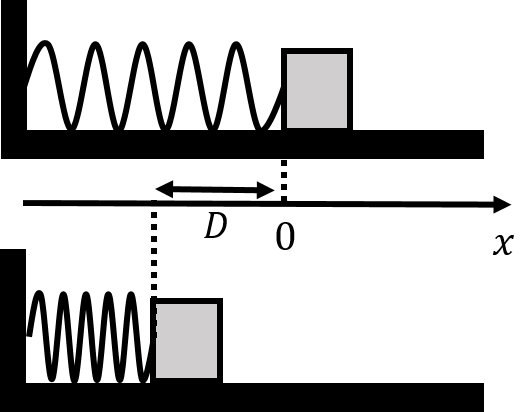
\includegraphics[width=0.4\linewidth]{files/blockspring-fdb4d8979bbf11d976ccd124d9539f46.png}
\caption[]{A block is launched along a frictionless surface by compressing a spring by a distance $D$. The top panel shows the spring when at rest, and the bottom panel shows the spring compressed by a distance $D$ just before releasing the block.}
\label{fig:applyingnewtonslaws:blockspring}
\end{figure}

A block of mass $m$ can slide freely along a frictionless surface. A horizontal spring, with spring constant, $k$, is attached to a wall on one end, while the other end can move freely, as shown in Figure~\ref{fig:applyingnewtonslaws:blockspring}. A coordinate system is defined such that the $x$ axis is horizontal and the free end of the spring is at $x=0$ when the spring is at rest. The block is pushed against the spring so that the spring is compressed by a distance $D$. The block is then released. What speed will the block have when it leaves the spring?

\begin{framed}
\textbf{Solution}\\
As you recall, the force exerted by a spring depends on the compression or extension of the spring and is given by Hooke's Law:
\begin{equation}
\vec F(x) = -kx\hat x
\end{equation}
where $x$ is the position of the free end of the spring and $x=0$ corresponds to the spring being at rest. In our case, when the edge of the block is located at $x_0= -D$ (the spring is compressed), the force is thus in the positive $x$ direction (since $x_0$ is a negative number).

The forces on the block are:

\begin{enumerate}
\item $\vec F_g$, its weight, with magnitude $mg$.
\item $\vec N$, a normal force exerted by the ground.
\item $\vec F(x)$, the spring force.
\end{enumerate}

Since the block is not moving vertically, the magnitude of the normal force must equal the weight $N=mg$, since these are the only forces with components in the vertical direction. The $x$ component of Newton's Second Law gives us the acceleration of the block (which depends on $x$):
\begin{equation}
\sum F_x = -kx &= ma(x)\\
\therefore a(x)&=-\frac{k}{m}x
\end{equation}
Again, recall that if $x$ is negative, then the acceleration will be in the positive direction. Since this scenario is exactly the same that we described above in the text, namely a force that varies continuously with position, we can apply the formula that we found earlier for determining the velocity after a varying force has been applied from position $x=x_0$ to position $x=X$:
\begin{equation}
V^2 &= v_0^2 + 2\int_{x_0}^{X}a(x)dx
\end{equation}
$V$ is the final speed that we would like to find, $v_0=0$ because the block starts at rest, and $x_0= -D$ is the starting position of the block. $X$ is the position along the $x$ axis where the block leaves the spring.

We have to think a little about what the value of $X$ should be: when the spring is compressed and the block accelerating, the spring is pushing the block in the positive $x$ direction. Once the block reaches $x=0$ the spring would want to pull the block backwards, but since it is not attached to the block, it stops exerting a force on the block at that point. The block thus leaves the spring at $x=0$, so that the final position is $X=0$. The speed of the block when it leaves the spring is thus:
\begin{equation}
V^2 &= v_0^2 + 2\int_{x_0}^{X}a(x)dx\\
&= 0 + 2\int_{-D}^{0}a(x)dx\\
&= 2\int_{-D}^{0}-\frac{k}{m}xdx\\
&= 2\left[ - \frac{k}{m}\frac{1}{2}x^2\right]_{-D}^{0}\\
&= \frac{k}{m}D^2\\
\therefore V &= \sqrt{\frac{k}{m}}D
\end{equation}
\textbf{Discussion:} This model for the speed of the block when it leaves the spring makes sense because:

\begin{itemize}
\item The dimension for the expression for $V$ is correct (you should check this!).
\item If the spring is compressed more (bigger value of $D$), then the speed will be higher.
\item If the mass is bigger (more inertia), then the final speed will be lower.
\item If the spring is stiffer (bigger value of $k$), then the final speed will be higher.
\end{itemize}

If you have studied physics before, you may have realized that the speed is easily found by conservation of energy:
\begin{equation}
\frac{1}{2}mV^2=\frac{1}{2}kD^2
\end{equation}
which gives the same value for $V$. As we will see in a later chapter, kinetic and potential energy are defined as they are, precisely because it makes using conservation of energy equivalent to using forces as we just did.
\end{framed}
\end{framed}

\begin{framed}
\textbf{Example 6.4}\\
An object of mass $m$ is released from rest out of a helicopter. The drag (air-resistance) on the object can be modelled as having a magnitude given by $bv$, where $v$ is the speed of the object and $b$ is a constant of proportionality. How does the velocity of the object depend on time?

\begin{framed}
\textbf{Solution}\\
As the object falls through the air, the forces exerted on the object are:

\begin{enumerate}
\item $F_g$, its weight, with magnitude $mg$, exerted downwards.
\item $F_d$, the force of drag, with magnitude $bv$, exerted upwards.
\end{enumerate}

Since the object will fall in a straight line, this is a one-dimensional problem, and we can choose the $x$ axis to be vertical, with positive $x$ pointing downwards, and the origin located where the object was released. The object will thus have a positive acceleration and move in the positive $x$ direction with this choice of coordinate system. This is illustrated in the free-body diagram in Figure~\ref{fig:applyingnewtonslaws:drag_fbd}.

\begin{figure}[!htbp]
\centering
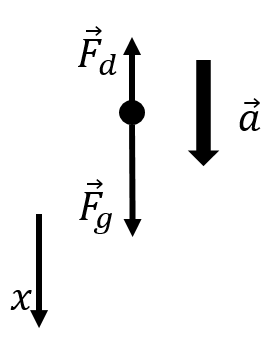
\includegraphics[width=0.2\linewidth]{files/drag_fbd-26e723b9982f949036c077b5eb8d1210.png}
\caption[]{Free-body diagram for a block free-falling with drag.}
\label{fig:applyingnewtonslaws:drag_fbd}
\end{figure}

Newton's Second Law for the object gives:
\begin{equation}
\sum F_x = F_g - F_d &= ma\\
mg - bv &= ma\\
\therefore a &= g-\frac{b}{m}v
\end{equation}
In this case, the acceleration depends explicitly on velocity rather than position, as we had before. However, we can use the same methodology to find how the velocity changes with time. First, we can note that the acceleration is zero if:
\begin{equation}
g-\frac{b}{m}v &=0\\
\therefore v = \frac{mg}{b}
\end{equation}
That is, once the object reaches a speed of $v_{term}=mg/b$, it will stop accelerating, i.e. it will reach ``terminal velocity''. Note that this is the same condition as requiring that the drag force ($bv$) have the same magnitude as the weight ($mg$).

Writing the acceleration as $a=\frac{dv}{dt}$, we can write:
\begin{equation}
\frac{dv}{dt} &= \left(g-\frac{b}{m}v \right)
\end{equation}
which again, is a separable differential equation, in which we can write the terms that depend on $v$ and those that depend on $t$ on separate sides of the equal sign:
\begin{equation}
\frac{dv}{g-\frac{b}{m}v}&= dt\\
\frac{dv}{v-\frac{mg}{b}}&= -\frac{b}{m}dt\\
\end{equation}
where we re-arranged the equation in the second line so that it would be easier to integrate in the next step. We can find the velocity, $v(t)$, at some time, $t$, by stating that $v=0$ at $t=0$ and taking the integrals (sum) on both sides. Again, we are modelling the motion as being made up of a large number of very small segments where the quantities on both sides of the equation are the same. Thus, if we sum (integrate) those quantities over all of the same segments, the left and right hand side of the equations will still be equal to each other:
\begin{equation}
\int_0^{v(t)}\frac{dv}{v-\frac{mg}{b}} &= -\int_0^t\frac{b}{m} dt\\
\left[\ln\left(v-\frac{mg}{b} \right)\right]_0^{v(t)} &=-\frac{b}{m}t\\
\ln\left(v(t)-\frac{mg}{b} \right)-\ln\left(-\frac{mg}{b} \right)&=-\frac{b}{m}t\\
\ln\left( \frac{v(t)-\frac{mg}{b}}{-\frac{mg}{b}} \right)&=-\frac{b}{m}t\\
\end{equation}
where, in the last line, we used the property that $\ln(a) -\ln(b)=\ln(a/b)$. By taking the exponential on either side of the equation ($e^{\ln(x)}=x$), we can find an expression for the velocity as a function of time:
\begin{equation}
\frac{v(t)-\frac{mg}{b}}{-\frac{mg}{b}} &= e^{-\frac{b}{m}t}\\
v(t)-\frac{mg}{b} &= -\frac{mg}{b}e^{-\frac{b}{m}t}\\
\therefore v(t) &= \frac{mg}{b}-\frac{mg}{b}e^{-\frac{b}{m}t}\\
&=\frac{mg}{b}\left(1-e^{-\frac{b}{m}t}\right)
\end{equation}
\textbf{Discussion:} This equation tells us that the velocity increases as a function of time, but the rate of increase decreases exponentially with time. At time $t=0$, the velocity is zero, as expected. As $t$ approaches infinity, $v$ approaches, $\frac{mg}{b}$, which is the terminal velocity. The time dependence of the velocity is illustrated in Figure~\ref{fig:applyingnewtonslaws:drag_vt}.

\begin{figure}[!htbp]
\centering
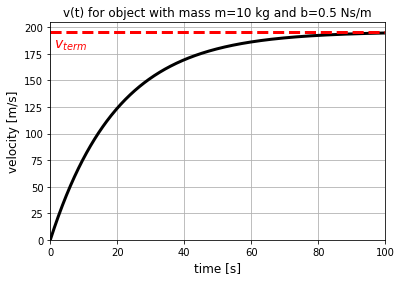
\includegraphics[width=0.7\linewidth]{files/drag_vt-801a0464afdbabb69c22a18071c30d9b.png}
\caption[]{Velocity as a function of time for an object of mass $m={\rm 10{kg}}$ which is free-falling from rest with a drag coefficient $b={\rm{0.5}{Ns/m}}$.}
\label{fig:applyingnewtonslaws:drag_vt}
\end{figure}
\end{framed}
\end{framed}

\subsubsection{Uniform circular motion}

As we saw in Section~\ref{chap:momentumandcm}, ``uniform circular motion'' is defined to be motion along a circle with constant speed. This may be a good time to review Section~\ref{sec:momentumandcm:circularmotion} for the kinematics of motion along a circle. In particular, for the uniform circular motion of an object around a circle of radius $R$, you should recall that:

\begin{itemize}
\item The velocity vector, $\vec v$, is always tangent to the circle.
\item The acceleration vector, $\vec a$, is always perpendicular to the velocity vector, because the magnitude of the velocity vector does not change.
\item The acceleration vector, $\vec a$, always points towards the centre of the circle.
\item The acceleration vector has magnitude $a=v^2/R$.
\item The angular velocity, $\omega$, is related to the magnitude of the velocity vector by $v=\omega R$ and is constant.
\item The angular acceleration, $\alpha$, is zero for uniform circular motion, since the angular velocity does not change.
\end{itemize}

In particular, you should recall that even if the speed is constant, the acceleration vector is always non-zero in uniform circular motion because the \textbf{velocity changes direction}. According to Newton's Second Law, this implies that there \textbf{must be a net force on the object that is directed towards the centre of the circle}\footnote{The sum of the forces is often called the ``net force'' on an object, and in the specific case of uniform circular motion, that net force is sometimes called the ``centripetal force'' - however, it is not a force in and of itself and it is always the sum of the forces that points towards the centre of the circle.} (parallel to the acceleration):
\begin{equation}
\sum \vec F = m\vec a
\end{equation}
where the acceleration has a magnitude $a=v^2/R$. Because the acceleration is directed towards the centre of the circle, we sometimes call it a ``radial'' acceleration (parallel to the radius), $a_R$, or a ``centripetal'' acceleration (directed towards the centre), $a_c$.

Consider an object in uniform circular motion in a horizontal plane on a frictionless surface, as depicted in Figure~\ref{fig:applyingnewtonslaws:circleH}.

\begin{figure}[!htbp]
\centering
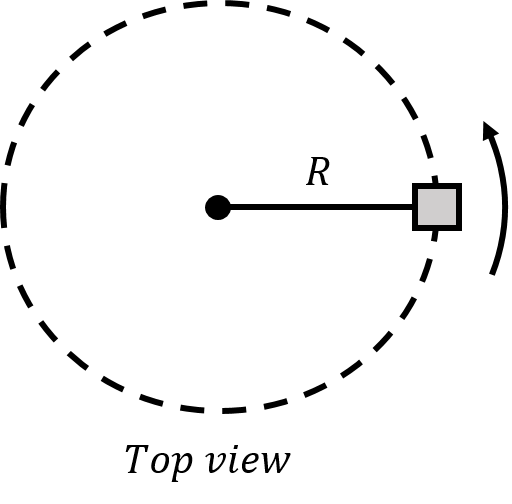
\includegraphics[width=0.3\linewidth]{files/circleH-14562d22cc39e77912bf057585173f4f.png}
\caption[]{An object undergoing uniform circular motion on a frictionless surface, as seen from above.}
\label{fig:applyingnewtonslaws:circleH}
\end{figure}

The only way for the object to undergo uniform circular motion as depicted is if the net force on the object is directed towards the centre of the circle. One way to have a force that is directed towards the centre of the circle is to attach a string between the center of the circle and the object, as shown in Figure~\ref{fig:applyingnewtonslaws:circleH}. If the string is under tension, the force of tension will always be towards the centre of the circle. The forces on the object are thus:

\begin{enumerate}
\item $\vec F_g$, its weight with magnitude $mg$.
\item $\vec N$, a normal forced exerted by the surface.
\item $\vec T$, a force of tension exerted by the string.
\end{enumerate}

The forces are depicted in the free-body diagram shown in Figure~\ref{fig:applyingnewtonslaws:circleH_fbd} (as viewed from the side), where we also drew the acceleration vector. Note that this free-body diagram is only ``valid'' at a particular instant in time since the acceleration vector continuously changes direction and would not always be lined up with the $x$ axis.

\begin{figure}[!htbp]
\centering
\begin{figure}[!htbp]
\centering
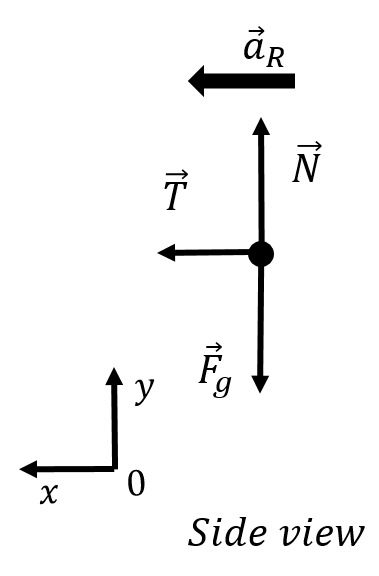
\includegraphics[width=0.25\linewidth]{files/circleH_fbd-9405d67831ff6d672f095e85893f0fec.png}
\caption[]{Free-body diagram (side view) for the object from [](\#fig:applyingnewtonslaws:circleH\_fbd)}
\label{fig:applyingnewtonslaws:circleH_fbd-a}
\end{figure}

\begin{figure}[h]
\centering
\begin{verbatim}
Writing out the $x$ and $y$ components of Newton's Second Law:
```{math}
\sum F_x &= T = ma_R\\
\sum F_y &= N - F_g =0
\end{verbatim}
\caption[]{}
\label{fig:applyingnewtonslaws:circleH_fbd-b}
\end{figure}
\caption[]{Free-body diagram (side view) for the object from Figure~\ref{fig:applyingnewtonslaws:circleH_fbd}}
\label{fig:applyingnewtonslaws:circleH_fbd-b}
\end{figure}

The $y$ component just tells us that the normal force must have the same magnitude as the weight because the object is not accelerating in the vertical direction. The $x$ component tells us the relation between the magnitudes of the tension in the string and the radial acceleration. Using the speed of the object, we can also write the relation between the tension and the speed:
\begin{equation}
T &= ma_R=m\frac{v^2}{R}\\
\end{equation}
Thus, we find that the tension in the string increases with the square of the speed, and decreases with the radius of the circle.

\begin{framed}
\textbf{Checkpoint}\\
\begin{figure}[!htbp]
\centering
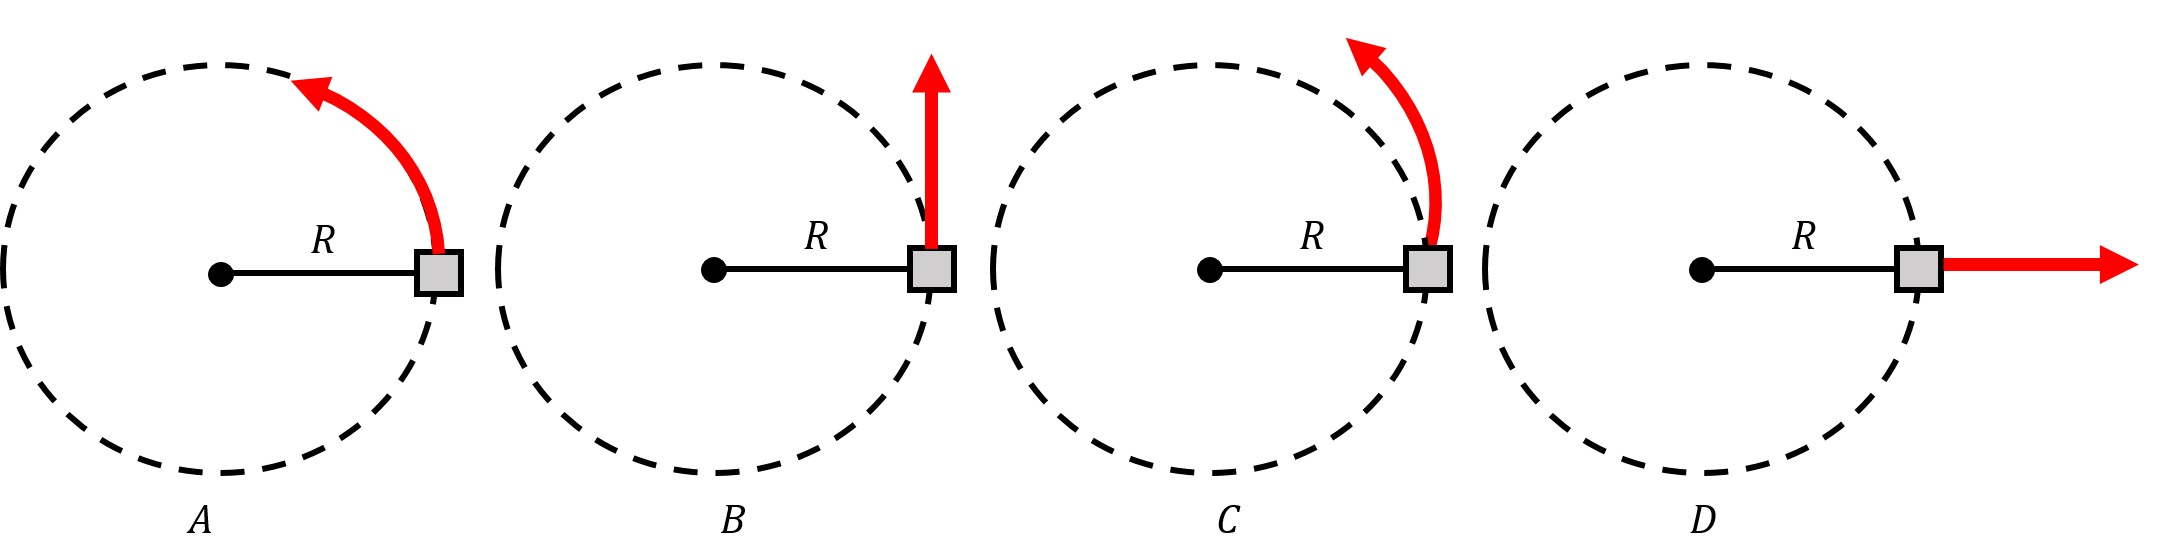
\includegraphics[width=0.9\linewidth]{files/trajectoryABCD-e53c5dce049569c31882a56f048ff7c1.png}
\caption[]{Possible trajectories (in red) that the block will follow if the string breaks.```
An object is undergoing uniform circular motion in the horizontal plane, when the string connecting the object to the centre of rotation suddenly breaks. What path will the block take after the string broke?

\begin{enumerate}
\item A
\item B
\item C
\item D
\end{enumerate}

\begin{framed}
\textbf{Answer}\\
\begin{enumerate}[resume]
\item
\end{enumerate}
\end{framed}}
\label{fig:applyingnewtonslaws:trajectoryABCD}
\end{figure}
\end{framed}

\begin{framed}
\textbf{Example 6.5}\\
\begin{figure}[!htbp]
\centering
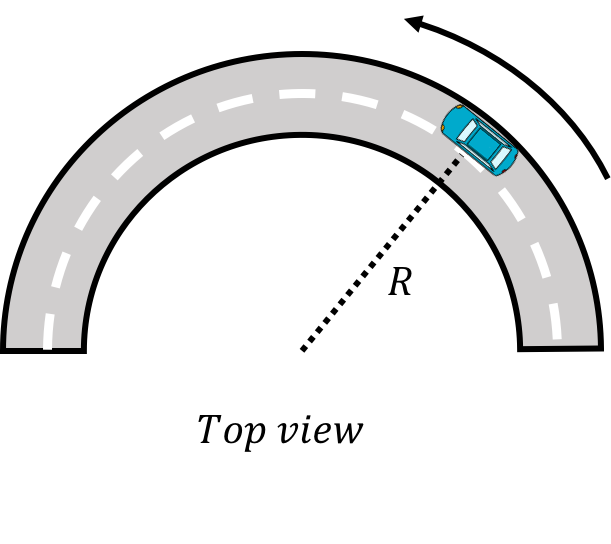
\includegraphics[width=0.25\linewidth]{files/car-bf4ad6e87eff6afa0747d345878e1215.png}
\caption[]{A car going around a curve that can be approximated as the arc of a circle of radius $R$.}
\label{fig:applyingnewtonslaws:car}
\end{figure}

A car goes around a curve which can be approximated as the arc of a circle of radius $R$, as shown in Figure~\ref{fig:applyingnewtonslaws:car}. The coefficient of static friction between the tires of the car and the road is $\mu_s$. What is the maximum speed with which the car can go around the curve without skidding?

\begin{framed}
\textbf{Solution}\\
If the car is going at constant speed around a circle, then the sum of the forces on the car must be directed towards the centre of the circle. The only force on the car that could be directed towards the centre of the circle is the force of friction between the tires and the road. If the road were perfectly slick (think driving in icy conditions), it would not be possible to drive around a curve since there could be no force of friction. The forces on the car are:

\begin{enumerate}
\item $\vec F_g$, its weight with magnitude $mg$.
\item $\vec N$, a normal force exerted upwards by the road.
\item $\vec f_s$, a force of static friction between the tires and the road. This is static friction, because the surface of the tire does not move relative to the surface of the road if the car is not skidding. The force of static friction has a magnitude that is at most $f_s\leq\mu_sN$.
\end{enumerate}

The forces on the car are shown in the free-body diagram in Figure~\ref{fig:applyingnewtonslaws:car_fbd}.

\begin{figure}[!htbp]
\centering
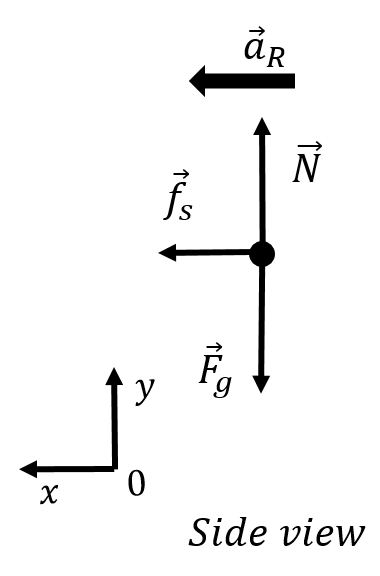
\includegraphics[width=0.25\linewidth]{files/car_fbd-13c36c93d0db1221ca48d0f4b097b1d4.png}
\caption[]{Free-body diagram for the car as seen looking at the car from the back (the centre of the curve is towards the left).}
\label{fig:applyingnewtonslaws:car_fbd}
\end{figure}

The $y$ component of Newton's Second Law tells us that the normal force exerted by the road must equal the weight of the car:
\begin{equation}
\sum F_y = N-F_g&=0\\
\therefore N &=mg
\end{equation}
The $x$ component relates the force of friction to the radial acceleration (and thus to the speed):
\begin{equation}
\sum F_x = f_s =ma_R&=m\frac{v^2}{R}\\
\therefore f_s &= m\frac{v^2}{R}
\end{equation}
The force of friction must be less than or equal to $f_s\leq\mu_sN=\mu_smg$ (since $N=mg$ from the $y$ component of Newton's Second Law), which gives us a condition on the speed:
\begin{equation}
f_s = m\frac{v^2}{R}&\leq\mu_smg\\
v^2 &\leq \mu_s g R\\
\therefore v &\leq \sqrt{\mu_s g R}
\end{equation}
Thus, if the speed is less than $\sqrt{\mu_s g R}$, the car will not skid and the magnitude of the force of static friction, which results in an acceleration towards the centre of the circle, will be smaller or equal to its maximal possible value.

\textbf{Discussion:} The model for the maximum speed that the car can travel around the curve makes sense because:

\begin{itemize}
\item The dimension of $\sqrt{\mu_s g R}$ is speed.
\item The speed is larger if the radius of the curve is larger (one can go faster around a wider curve without skidding).
\item The speed is larger if the coefficient of friction is large (if the force of friction is larger, a larger radial acceleration can be sustained).
\end{itemize}
\end{framed}
\end{framed}

\begin{framed}
\textbf{Example 6.6}\\
\begin{figure}[!htbp]
\centering
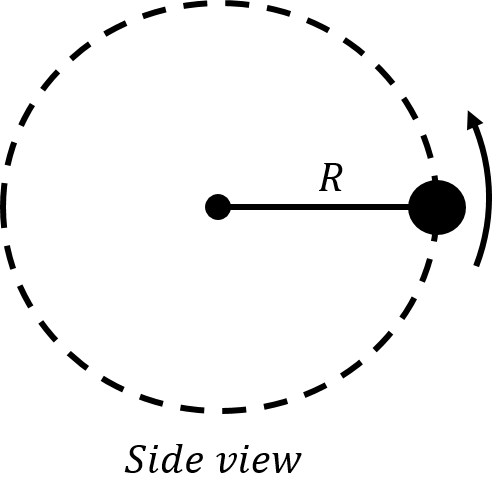
\includegraphics[width=0.27\linewidth]{files/circleV-e337f1c803dda6f492d5f1f0b409191b.png}
\caption[]{A ball attached to a string undergoing circular motion in a vertical plane.}
\label{fig:applyingnewtonslaws:circleV}
\end{figure}

A ball is attached to a mass-less string and executing circular motion along a circle of radius $R$ that is in the vertical plane, as depicted in Figure~\ref{fig:applyingnewtonslaws:circleV}. Can the speed of the ball be constant? What is the minimum speed of the ball at the top of the circle if it is able to make it around the circle?

\begin{framed}
\textbf{Solution}\\
The forces that are acting on the ball are:

\begin{enumerate}
\item $\vec F_g$, its weight with magnitude $mg$.
\item $\vec T$, a force of tension exerted by the string.
\end{enumerate}

Figure~\ref{fig:applyingnewtonslaws:circleV_fbd} shows the free-body diagram for the forces on the ball at three different locations along the path of the circle.

\begin{figure}[!htbp]
\centering
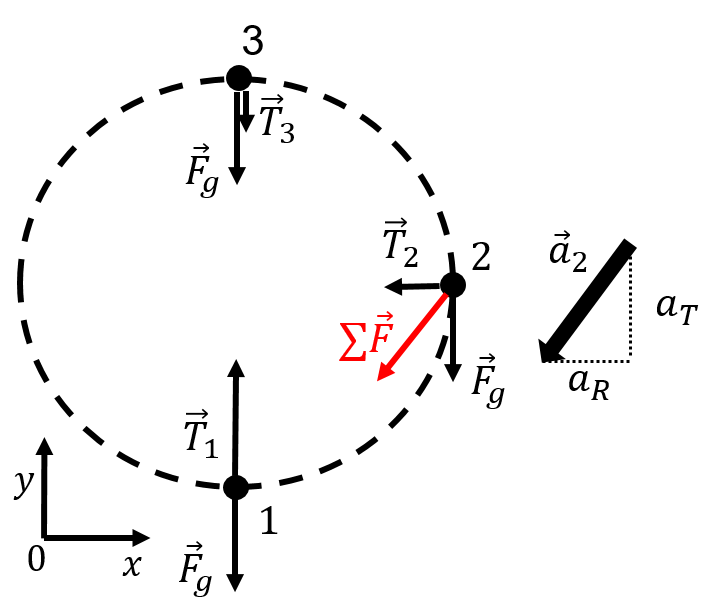
\includegraphics[width=0.4\linewidth]{files/circleV_fbd-ffbc3de10018feef97a6cd6d4f6adba4.png}
\caption[]{A ball attached to a string undergoing circular motion in a vertical plane.}
\label{fig:applyingnewtonslaws:circleV_fbd}
\end{figure}

In order for the ball to go around in a circle, there must be at least a component of the net force on the ball that is directed towards the centre of the circle at all times. In the bottom half of the circle (positions 1 and 2), only the tension can have a component directed towards the centre of the circle.

Consider in particular the position labelled 2, when the string is horizontal and the tension is equal to $\vec T_2$. The free-body diagram in Figure~\ref{fig:applyingnewtonslaws:circleV_fbd} also shows the vector sum of the weight and tension at position 2 (the red arrow labelled $\sum \vec F$), which points downwards and to the left. It is thus clearly impossible for the acceleration vector to point towards the centre of the circle, and the acceleration will have components that are both tangential ($a_T$) to the circle and radial ($a_R$), as shown by the vector $\vec a_2$ in Figure~\ref{fig:applyingnewtonslaws:circleV_fbd}.

The radial component of the acceleration will change the direction of the velocity vector so that the ball remains on the circle, and the tangential component will reduce the magnitude of the velocity vector. According to our model, it is thus impossible for the ball to go around the circle at constant speed, and the speed must decrease as it goes from position 2 to position 3, no matter how one pulls on the string (you can convince yourself of this by drawing the free-body diagram at any point between points 2 and 3).

The minimum speed for the ball at the top of the circle is given by the condition that the tension in the string is zero just at the top of the trajectory (position 3). The ball can still go around the circle because, at position 3, gravity is towards the centre of the circle and can thus give an acceleration that is radial, even with no tension. The $y$ component of Newton's Second Law, at position 3 gives:
\begin{equation}
\sum F_y = -F_g &= ma_y\\
\therefore a_y &=-g
\end{equation}
The magnitude of the acceleration is the radial acceleration, and is thus related to the speed at the top of the trajectory:
\begin{equation}
a_R&=-a_y=g = \frac{v^2}{R}\\
\therefore v_{min}&=\sqrt{gR}
\end{equation}
which is the minimum speed at the top of the trajectory for the ball to be able to continue along the circle. The tension in the string would change as the ball moves around the circle, and will be highest at the bottom of the trajectory, since the tension has to be bigger than gravity so that the net force at the bottom of the trajectory is upwards (towards the centre of the circle).

\textbf{Discussion:} The model for the minimum speed of the ball at the top of the circle makes sense because:

\begin{itemize}
\item $\sqrt{gR}$ has the dimension of speed.
\item The minimum velocity is larger if the circle has a larger radius (try this with a mass attached at the end of a string).
\item The minimum velocity is larger if the mass is bigger (again, try this at home!).
\end{itemize}
\end{framed}
\end{framed}

\begin{framed}
\textbf{Checkpoint}\\
Consider a ball attached to a string, being spun in a vertical circle (such as the one depicted in Figure~\ref{fig:applyingnewtonslaws:circleV}). If you shortened the string, how would the minimum angular velocity (measured at the top of the trajectory) required for the ball to make it around the circle change?

\begin{enumerate}
\item It would decrease
\item It would stay the same
\item It would increase
\end{enumerate}

\begin{framed}
\textbf{Answer}\\
\begin{enumerate}
\item
\end{enumerate}
\end{framed}
\end{framed}

\paragraph{Banked curves}

As we saw in Example~6.5, there is a maximum speed with which a car can go around a curve before it starts to skid. You may have noticed that roads, highways especially, are banked where there are curves. Racetracks for cars that go around an oval (the boring kind of car races) also have banked curves. As we will see, this allows the speed of vehicles to be higher when going around the curve; or rather, it makes the curves safer as the speed at which vehicles \textit{would} skid is higher. In Example~6.5, we saw that it was the force of static friction between the tires of the car and the road that provided the only force with a component towards the centre of the circle. The idea of using a banked curve is to change the direction of the normal force between the road and the car tires so that it, too, has a component in the direction towards the centre of the circle.

Consider the car depicted in Figure~\ref{fig:applyingnewtonslaws:carbank} which is seen from behind making a left turn around a curve that is banked by an angle $\theta$ with respect to the horizontal and can be modelled as an arc from a circle of radius $R$.

\begin{figure}[!htbp]
\centering
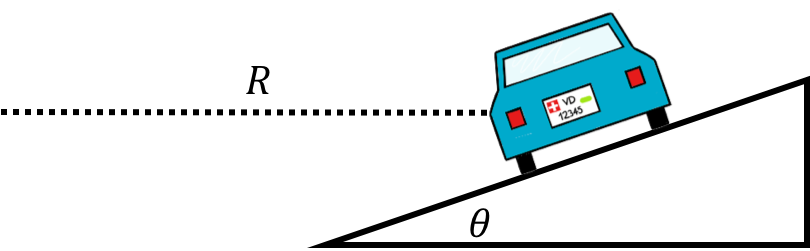
\includegraphics[width=0.7\linewidth]{files/carbank-1f87f47046a3d7845d4293aeb68f4429.png}
\caption[]{A car moving into the page and going around a banked curved so that it is turning towards the left (the centre of the circle is to the left).}
\label{fig:applyingnewtonslaws:carbank}
\end{figure}

The forces exerted on the car are the same as in Example~6.5, except that they point in different directions. The forces are:

\begin{enumerate}
\item $\vec F_g$, its weight with magnitude $mg$.
\item $\vec N$, a normal force exerted by the road, perpendicular to the surface of the road.
\item $\vec f_s$, a force of static friction between the tires and the road. This is static friction, because the surface of the tire does not move relative to the surface of the road if the car is not skidding. The force of static friction has a magnitude that is at most $f_s\leq\mu_sN$ and is perpendicular to the normal force. The force could be either upwards or downwards, \textit{depending on the other forces on the car}.
\end{enumerate}

A free-body diagram for the forces on the car is shown in Figure~\ref{fig:applyingnewtonslaws:carbank_fbd}, along with the acceleration (which is in the radial direction, towards the centre of the circle), and our choice of coordinate system (choosing $x$ parallel to the acceleration). The direction of the force of static friction is not known \textit{a priori} and depends on the speed of the car:

\begin{itemize}
\item If the speed of the car is zero, the force of static friction is upwards. With a speed of zero, the radial acceleration is zero, and the sum of the forces must thus be zero. The impeding motion of the car would be to slide down the banked curve (just like a block on an incline).
\item If the speed of the car is very large, the force of static friction is downwards, as the impeding motion of the car would be to slide up the bank. The natural motion of the car is to go in a straight line (Newton's First Law). If the components of the normal force and of the force of static friction directed towards the centre of the circle are too small to allow the car to turn, then the car would slide up the bank (so the impeding motion is up the bank and the force of static friction is downwards).
\end{itemize}

\begin{figure}[!htbp]
\centering
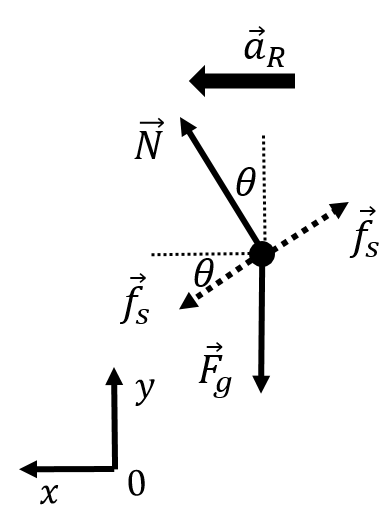
\includegraphics[width=0.3\linewidth]{files/carbank_fbd-abf6ccb44dd218cc25f1a2b082e9acd0.png}
\caption[]{Free-body diagram for the forces on the car. The direction of the force of static friction cannot be determined, as it depends on the acceleration of the car, so it is shown twice (with dotted lines).}
\label{fig:applyingnewtonslaws:carbank_fbd}
\end{figure}

There is thus an ``ideal speed'' at which the force of static friction is precisely zero, and the $x$ component of the normal force is responsible for the radial acceleration. At higher speeds, the force of static friction is downwards and increases in magnitude to keep the car's acceleration towards the centre of the circle. At some maximal  speed, the force of friction will reach its maximal value, and no longer be able to keep the car's acceleration pointing towards the centre of the circle. At speeds lower than the ideal speed, the force of friction is directed upwards to prevent the car from sliding down the bank. If the coefficient of static friction is too low, it is possible that at low speeds, the car would start to slide down the bank (so there would be a minimum speed below which the car would start to slide down).

Let us model the situation where the force of static friction is identically zero so that we can determine the ideal speed for the banked curve. The only two forces on the car are thus its weight and the normal force. The $x$ and $y$ component of Newton's Second Law give:
\begin{equation}
\label{eq:applyingnewtonslaws:carbank_x}
\sum F_x &= N\sin\theta = ma_R=m\frac{v^2}{R}\nonumber\\
\therefore N\sin\theta &= m\frac{v^2}{R}
\end{equation}
\begin{equation}
\label{eq:applyingnewtonslaws:carbank_y}
\sum F_y &= N\cos\theta-F_g = 0\nonumber\\
\therefore N\cos\theta&=mg
\end{equation}
We can divide Equation (\ref{eq:applyingnewtonslaws:carbank_x}) by Equation (\ref{eq:applyingnewtonslaws:carbank_y}), noting that $\tan\theta=\sin\theta/\cos\theta$, to obtain:
\begin{equation}
\tan\theta &= \frac{v^2}{gR}\\
\therefore v_{ideal} &=\sqrt{gR\tan\theta}
\end{equation}
At this speed, the force of static friction is zero. In practice, one would use this equation to determine which bank angle to use when designing a road, so that the ideal speed is around the speed limit or the average speed of traffic. We leave it as an exercise to determine the maximal speed that the car can go around the curve before sliding out.

\paragraph{Inertial forces in circular motion}

As you sit in a car that is going around a curve, you will feel pushed outwards, away from the centre of the circle that the car is going around. This is because of your inertia (Newton's First Law), and your body would go in a straight line if the car were not exerting a net force on you towards the centre of the circle. You are not so much feeling a force that is pushing you outwards as you are feeling the effects of the car seat pushing you inwards; if you were leaning against the side of the car that is on the outside of the curve, you would feel the side of the car pushing you inwards towards the centre of the curve, even if it ``feels'' like you are pushing outwards against the side of the car.

If we model your motion looking at you from the ground, we would include a force of friction between the car seat (or the side of the car, or both) and you that is pointing towards the centre of the circle, so that the sum of the forces exerted on you is towards the centre of the circle. We can also model your motion from the non-inertial frame of the car. As you recall, because this is a non-inertial frame of reference, we need to include an additional inertial force, $\vec F_I$, that points opposite of the acceleration of the car, with magnitude $F_I=ma_R$ (if the net acceleration of the car is $a_R$). Inside the non-inertial frame of reference of the car, your acceleration (relative to the reference frame, i.e. the car) is zero. This is illustrated by the diagrams in Figure~\ref{fig:applyingnewtonslaws:carinertial}.

\begin{figure}[!htbp]
\centering
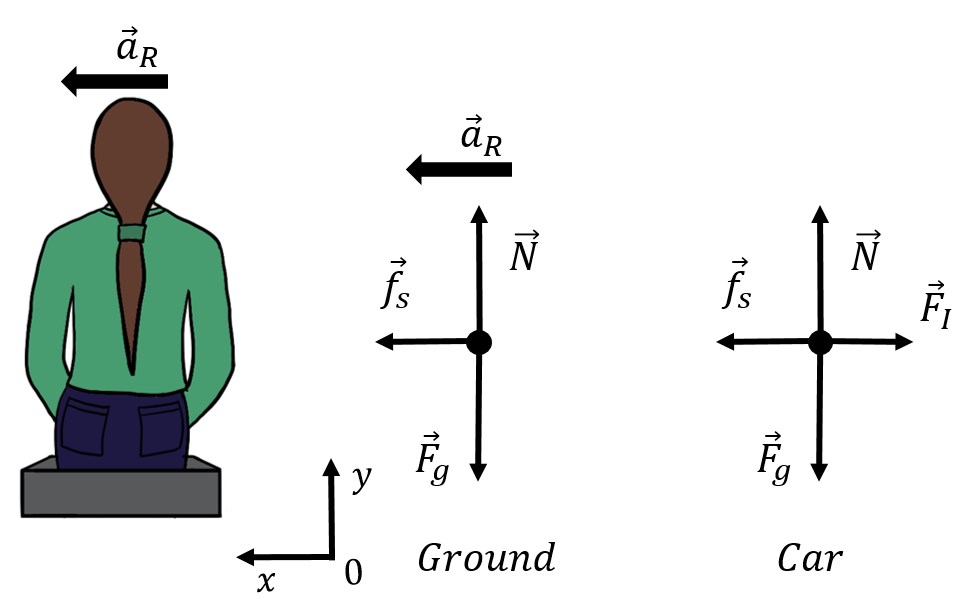
\includegraphics[width=0.6\linewidth]{files/carinertial-f8a601732d9a4618a143e7df196a197c.png}
\caption[]{(Left:) A person sitting on a car seat in a car turning towards the left. (Centre:) Free-body diagram for the person as modelled in the inertial reference frame of the ground. (Right:) Free-body diagram for the person as modelled in the non-inertial frame of reference of the car, including an additional inertial force.}
\label{fig:applyingnewtonslaws:carinertial}
\end{figure}

The $y$ component of Newton's Second Law in both frames of reference is the same:
\begin{equation}
\sum F_y&=N-F_g=0\\
\therefore N&=mg
\end{equation}
and simply tells us that the normal force is equal to the weight. In the reference frame of the ground, the $x$ component of Newton's Second Law gives:
\begin{equation}
\sum F_x &= f_s = ma_R\\
\therefore f_s &= m\frac{v^2}{R}
\end{equation}
In the frame of reference of the car, where your acceleration is zero and an inertial force of magnitude $F_I=mv^2/R$ is exerted on you, the $x$ component of Newton's Second Law gives:
\begin{equation}
\sum F_x &= f_s-F_I = 0\\
\therefore f_s - m\frac{v^2}{R} &= 0
\end{equation}
which of course, mathematically, is exactly equivalent. The inertial force is not a real force in the sense that it is not exerted by anything. It only comes into play because we are trying to use Newton's Laws in a non-inertial frame of reference. However, it does provide a good model for describing the sensation that we have of being pushed outwards when the car goes around a curve. Sometimes, people will refer to this force as a ``centrifugal'' force, which means ``a force that points away from the centre''. You should however remember that this is not a real force exerted on the object, but is the result of modelling motion in a non-inertial frame of reference.

\begin{framed}
\textbf{Checkpoint}\\
Jamie is driving his tricycle around a circular pond. Jamie feels a centrifugal force with magnitude $F_I$. If Jamie pedals twice as fast, what will be the magnitude of the centrifugal force that he experiences?

\begin{enumerate}
\item $\sqrt{2}F_I$
\item $\frac{1}{2}F_I$
\item $2F_I$
\item $4F_I$
\end{enumerate}

\begin{framed}
\textbf{Answer}\\
\begin{enumerate}[resume]
\item
\end{enumerate}
\end{framed}
\end{framed}

\subsubsection{Non-uniform circular motion}

In non-uniform circular motion, an object's motion is along a circle, but the object's speed is not constant. In particular, the following will be true

\begin{itemize}
\item The object's velocity vector is always tangent to the circle.
\item The speed and angular speed of the object are not constant.
\item The angular acceleration of the object is not zero.
\item The acceleration vector will not point towards the centre of the circle.
\end{itemize}

Since the acceleration vector does not point towards the centre of the circle, it is usually convenient to break up the acceleration vector into two components: $a_R$, a component that is radial (towards the centre of the circle), and $a_T$, a component that is tangent to the circle (and perpendicular to to the radial component). The \textbf{radial component is ``responsible'' for the change in direction of the velocity} such that the object goes in a circle. the magnitude of the radial acceleration is the same as it is for uniform circular motion:
\begin{equation}
a_R=\frac{v^2}{r}
\end{equation}
where the speed is no longer constant in time. The tangential component of the acceleration is responsible for changing the magnitude of the velocity of the object:
\begin{equation}
a_T = \frac{dv}{dt}
\end{equation}

\begin{framed}
\textbf{Example 6.7}\\
\begin{figure}[!htbp]
\centering
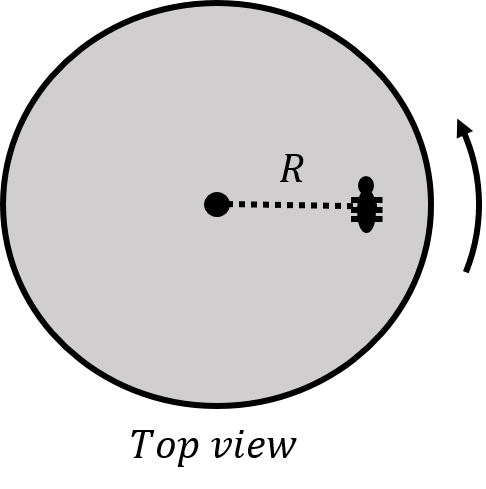
\includegraphics[width=0.25\linewidth]{files/ant-84c9202e5ee7cd9f6a0b3c1225f898dd.png}
\caption[]{An ant on a horizontal turntable that is starting to spin, as seen from above.}
\label{fig:applyingnewtonslaws:ant}
\end{figure}

A small ant is sleeping on a turntable just as the turntable starts to spin from rest, with an angular acceleration $\alpha=1 {\rm rad/s^2}$ that is small enough so that, initially, the ant remains on the turntable. The ant is a distance $R=0.1 {\rm m}$ from the centre of the turntable, as shown in Figure~\ref{fig:applyingnewtonslaws:ant}  and the coefficient of static friction between the ant's ``feet'' and the turntable is $\mu_s=0.5$. After how much time will the ant slide off from the turntable?

\begin{framed}
\textbf{Solution}\\
As the turntable accelerates, the force of static friction between the turntable and the ant will keep the ant moving with the turntable. Once the turntable is going fast enough, the force of friction will no longer be large enough to provide the total acceleration that is required to keep the ant moving with the turntable (with a constant tangential component of the acceleration and an increasing radial component of the acceleration).

The forces on the ant are:

\begin{enumerate}
\item $\vec F_g$, its weight, with magnitude $mg$.
\item $\vec N$, a normal force exerted by the turntable on the ant.
\item $\vec f_s$, a force of static friction exerted by the turntable on the ant. The force of friction will be such that it has both radial and tangential components.
\end{enumerate}

A free-body diagram for the forces on the ant is shown in Figure~\ref{fig:applyingnewtonslaws:ant_fbd}, as seen from above and from the side, for some point in time. We have chosen the point in time to be just when the ant is about to slide off of the turntable, when the force of static friction makes an unknown angle $\theta$ with the $x$ axis. We have placed the origin of the coordinate system at the centre of the turntable and chosen the $x$ axis such that the ant is located on the positive $x$ axis with its velocity in the positive $y$ direction. We used a three dimensional coordinate system where the weight and normal force are exerted in the $z$ (vertical) direction since the acceleration vector of the ant will have both radial ($x$) and tangential ($y$) components.

\begin{figure}[!htbp]
\centering
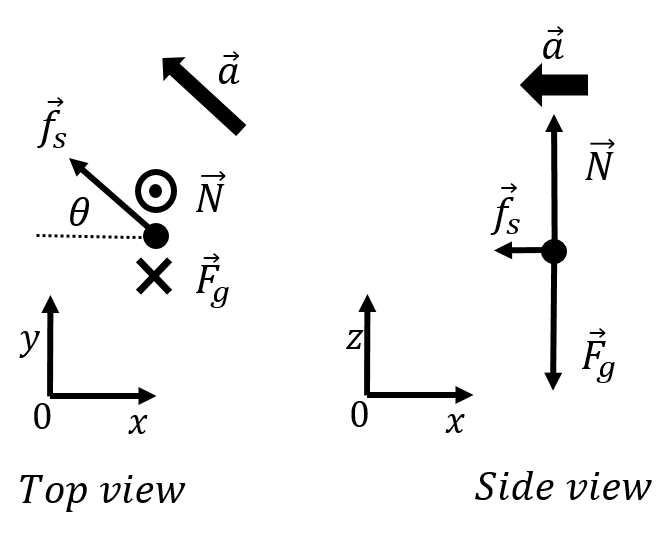
\includegraphics[width=0.5\linewidth]{files/ant_fbd-57dca3079c2f89aaf00fa3c11af1f13f.png}
\caption[]{(Left:) Forces on the ant as seen from above. The normal force is out of the page ($\odot$), whereas the weight is into the page ($\times$). (Right:) Forces on the ant as seen from the side. Note that the acceleration vector and force of static friction also have components in the $y$ direction, which is why their magnitude is shown as being smaller than in the top view.}
\label{fig:applyingnewtonslaws:ant_fbd}
\end{figure}

Newton's Second Law has to be written out in three components. The $z$ component relates the weight and normal force:
\begin{equation}
\sum F_z &= N - F_g = 0\\
\therefore N&=mg
\end{equation}
The $x$ component of Newton's Second Law is such that the $x$ component of the acceleration is its radial component:
\begin{equation}
\sum F_x &= -f_s\cos\theta = -ma_R = -m\frac{v^2}{R}\\
\therefore f_s\cos\theta &= m\frac{v^2}{R}
\end{equation}
The $y$ component of Newton's Second Law relates the tangential component of the force of static friction to the tangential component of the acceleration:
\begin{equation}
\sum F_y &= f_s\sin\theta = ma_T \\
\therefore f_s\sin\theta &= m\alpha R
\end{equation}
where we used the fact that the (linear) tangential acceleration, $a_T$, is related to the angular acceleration, $\alpha$, by:
\begin{equation}
a_T = \alpha R
\end{equation}
Summarizing the three equations that we obtained from the three components of Newton's Second Law:
\begin{equation}
f_s\cos\theta &= m\frac{v^2}{R}\\
f_s\sin\theta &= m\alpha R\\
N&=mg
\end{equation}
Also, note that the speed, $v(t)$ at some time $t$ is given by simple kinematics:
\begin{equation}
v(t)=v_0+a_Tt=(0)+\alpha R t
\end{equation}
The ant will start to slip when the force of friction reaches its maximal amplitude, $f_s=\mu_sN=\mu_Smg$. The $x$ of Newton's Second Law can be used to find an expression for the time at which force of friction reaches its maximal value (in terms of the unknown angle $\theta$):
\begin{equation}
f_s\cos\theta &= m\frac{v^2}{R}\\
\mu_sg\cos\theta &= R\alpha^2t^2\\
\therefore t &= \sqrt{\frac{\mu_sg\cos\theta}{R\alpha^2}}
\end{equation}
We can use the $y$ component to determine the angle $\theta$:
\begin{equation}
f_s\sin\theta &= m\alpha R\\
\mu_sg\sin\theta &= \alpha R\\
\therefore \sin\theta &= \frac{\alpha R}{\mu_s g}\\
\therefore \theta &= \sin^{-1}\left( \frac{\alpha R}{\mu_s g}  \right)=\sin^{-1}\left( \frac{(1 {\rm rad/s^2})(0.1 {\rm m})}{(0.5)(9.8 {\rm N/kg})}  \right)\\
&=1.17 {\rm \degree}
\end{equation}
The angle is very small, and we see that the force of friction is mostly directed towards the centre of the circle. The radial acceleration is thus much larger than the tangential acceleration. We can then use the angle to find the time using the expression we derived above:
\begin{equation}
t &= \sqrt{\frac{\mu_sg\cos\theta}{R\alpha^2}}= \sqrt{\frac{(0.5)(9.8 {\rm N/kg})\cos(1.17 {\rm \degree})}{(0.1 {\rm m})(1 {\rm rad/s^2})^2}}\\
&=7.0 {\rm s}
\end{equation}
\end{framed}
\end{framed}

\subsubsection{Summary}

When the velocity of an object does not change direction continuously (``linear motion''), we can model its motion independently over several segments in such a way that the motion is one dimensional in each segment. This allows us to choose a coordinate system in each segment where the acceleration vector is co-linear with one of the axes.

When the forces on an object changes continuously, we need to use calculus to determine the motion of the object. If the velocity vector for an object changes direction continuously, we need to model the motion in each dimension independently.

If an object undergoes uniform circular motion, the acceleration vector and the sum of the forces always point towards the centre of the circle. In the radial direction, Newton's Second Law gives
\begin{equation}
\sum \vec F = ma_R = m\frac{v^2}{R}
\end{equation}
If an object's speed is changing as it moves around a circle the acceleration vector will have a component that is towards the centre of the circle (the radial component) and a component that is tangential to the circle. The tangential component is responsible for the change in speed, whereas the radial component is responsible for the change in direction of the velocity.

In a reference frame that is rotating about a circle, an inertial force, sometimes called the centrifugal force, appears to push all objects co-moving with the reference frame towards the outside of the circle.

\subsubsection{Thinking about the material}

\begin{framed}
\textbf{Reflect and research}\\
\begin{itemize}
\item Is there a maximum speed with which an object can spin? (Something about the thing eventually flying apart if it rotates too fast, as the atoms can not be held together at some point - maybe there is a cool video to look up?)
\end{itemize}
\end{framed}

\begin{framed}
\textbf{To try at home}\\
\begin{itemize}
\item Spin a mass on a string in a vertical circle, what is the tension in the string when the mass is at the top for it to barely make it around?
\item Spin a mass on a string in a vertical circle, how does the minimum speed at the top of the circle to barely make it around  depend on the radius of the circle or the mass?
\item Spin a mass on a string in a vertical circle, describe the motion if the mass does not have the minimum speed to make it around the circle. If it makes it to the top, does it automatically make it all the way around the circle?
\end{itemize}
\end{framed}

\begin{framed}
\textbf{To try in the lab}\\
\begin{itemize}
\item Build a conical pendulum and determine whether the opening angle of the cone is related to the speed of the bob, in the way that you expect it to be.
\item Propose an experiment to determine the effects of the drag force on projectile motion.
\item Propose an experiment which investigates an object's motion when placed on a spinning turntable.
\end{itemize}
\end{framed}

\subsubsection{Sample problems and solutions}

\paragraph{Problems}

\begin{framed}
\textbf{Problem 6.1}\\
Consider a conical pendulum with a mass $m$, attached to a string of length $L$. The mass executes uniform circular motion in the horizontal plane, about a circle of radius $R$, as shown in Figure~\ref{fig:applyingnewtonslaws:conicalpendulum}. One can think of the horizontal circle and the point where the string is attached to as forming a cone. The circular motion is such that the (constant) angle between the string and the vertical is $\theta$.

\begin{itemize}
\item a. Derive an expression for the tension in the string.
\item b.  Derive an expression for the speed of the mass.
\item c. Derive an expression for the period of the motion.
\end{itemize}

\begin{figure}[!htbp]
\centering
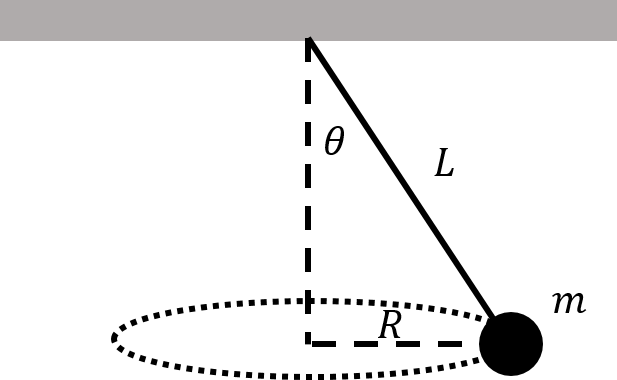
\includegraphics[width=0.3\linewidth]{files/conicalpendulum-909c2cb489ad7ac70f1f338395013c5c.png}
\caption[]{The conical pendulum.}
\label{fig:applyingnewtonslaws:conicalpendulum}
\end{figure}
\end{framed}

\begin{framed}
\textbf{Problem 6.2}\\
Barb and Kenny are going to the amusement park. Barb insists on riding the giant roller coaster, but Kenny is scared that they will fall out of the roller coaster at the top of the loop. Barb reassures Kenny by asking the roller coaster technician for more information. The technician says that they will be travelling at $15 {\rm m/s}$ when upside down, and that the roller coaster loop has a radius of $22 {\rm m}$. Kenny is still sceptical. Is he correct in being sceptical?

\begin{figure}[!htbp]
\centering
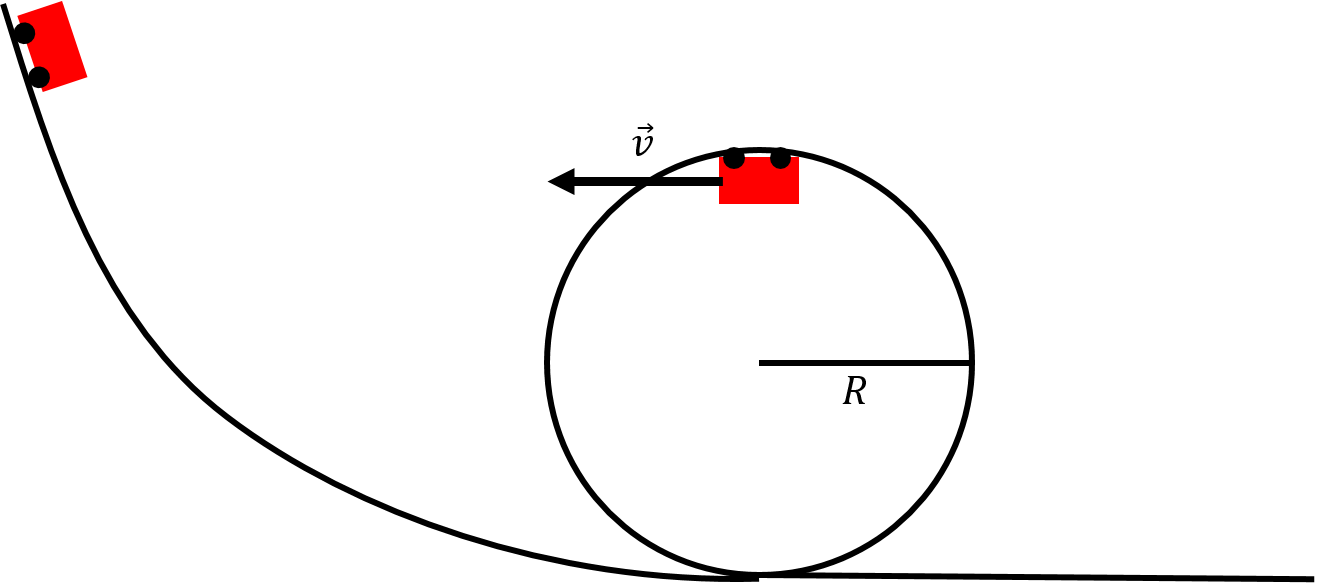
\includegraphics[width=0.6\linewidth]{files/rollercoaster-fcc6a55ec109e24ec90fcc064e2b34a0.png}
\caption[]{The roller coaster}
\label{fig:applyingnewtonslaws:rollercoaster}
\end{figure}
\end{framed}

\paragraph{Solutions}

\begin{framed}
\textbf{Solution 6.1}\\
\begin{itemize}
\item a. We start by identifying the forces that are acting on the mass. These are:
\item $\vec F_g$, its weight, with a magnitude $mg$.
\item $\vec F_T$, a force of tension exerted by the string.
\end{itemize}

The forces are illustrated in Figure~\ref{fig:applyingnewtonslaws:conicalpendulumfbd}, along with our choice of coordinate system and the direction of the acceleration of the mass (towards the centre of the circle).

\begin{figure}[!htbp]
\centering
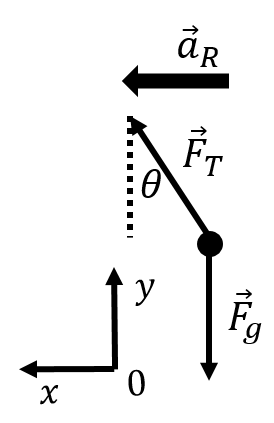
\includegraphics[width=0.2\linewidth]{files/conicalpendulumfbd-260518c853b0cc2419d64f256277bb48.png}
\caption[]{Forces acting on the conical pendulum}
\label{fig:applyingnewtonslaws:conicalpendulumfbd}
\end{figure}

The $y$ component of Newton's Second law gives the relation between the tension in the string, the weight, and the angle $\theta$
\begin{equation}
\sum F_y&=0 \\
F_T\cos\theta -F_g&=0 \\
F_T\cos\theta&=mg \\
\therefore F_T&=\frac{mg}{\cos\theta} \\
\end{equation}
\begin{itemize}
\item b. In order for the mass to move in a circle, the net force must be directed towards the centre of the circle at all times. The $x$ component of Newton's Second Law, combined with our expression for the magnitude of the tension, $F_T$, allows us to determine the speed of the mass:
\end{itemize}
\begin{equation}
\sum F_x&=ma_r \\
F_T\sin\theta&=m\frac{v^2}{R}\\
\left(\frac{mg}{\cos\theta}\right)\sin\theta &=m\frac{v^2}{R}\\
g\tan\theta&=\frac{v^2}{R}\\
\therefore v &= \sqrt{gR\tan\theta}
\end{equation}
\begin{itemize}
\item c. Now that we know the speed, we can easily find the period, $T$, of the motion:
\end{itemize}
\begin{equation}
T&=\frac{2\pi R}{v} \\
&=\frac{2\pi R}{\sqrt{gR\tan\theta }}=2\pi\sqrt{\frac{R}{g\tan\theta}}
\end{equation}
\end{framed}

\begin{framed}
\textbf{Solution 6.2}\\
We need to determine if the speed of Barb and Kenny is large enough for them to go around the circle. The minimum speed that they must have at the top of the loop is such that their weight (the only force acting on them) provides the centripetal (net) force required to go around the loop.

Writing Newton's Second Law in the vertical direction, for the case where only the weight acts on Barb or Kenny (mass $m$), when they are going at speed $v$
\begin{equation}
mg &= ma_R = m\frac{v^2}{R}\\
\therefore v &= \sqrt{gR} = \sqrt{(9.8 {\rm m/s^2})(22 {\rm m})}=14.68 {\rm m/s}
\end{equation}
This corresponds to the minimum speed that they must have at the top of the loop to make it around. If they go faster, the normal force from their seat (downwards, since they are upside-down), would result in a larger net force towards the centre of the circle. This situation corresponds to the normal force from their seat just barely reaching 0 at the top of the loop. Since the roller coaster is quoted as having a speed of $15 {\rm m/s}$ at the top of the loop, they will just barely make it. However, this is way too close to the minimal speed to not fall out of the roller coaster, so Kenny is correct in being sceptical! The engineers designing the roller coaster should include a much bigger safety margin!
\end{framed}